%\documentclass[times, 11pt, onecolumn]{article} 
%\documentclass[times, 10pt]{article} 
%\documentclass{article} 

\documentclass[conference,final]{IEEEtran}

\usepackage{latex8}
\usepackage{times}

\usepackage[utf8]{inputenc}
\usepackage{graphicx}
\usepackage{url}
\usepackage{float}
\usepackage{times}    
\usepackage{multirow}    
\usepackage{listings}   
\usepackage{times}     
\usepackage{paralist}    
\usepackage{wrapfig}    
\usepackage[small,it]{caption}
\usepackage{multirow}
\usepackage{ifpdf}
\usepackage{subfigure}

\usepackage{listings}
\usepackage{keyval}  
\usepackage{color}
\definecolor{listinggray}{gray}{0.95}
\definecolor{darkgray}{gray}{0.7}
\definecolor{commentgreen}{rgb}{0, 0.4, 0}
\definecolor{darkblue}{rgb}{0, 0, 0.4}
\definecolor{middleblue}{rgb}{0, 0, 0.7}
\definecolor{darkred}{rgb}{0.4, 0, 0}
\definecolor{brown}{rgb}{0.5, 0.5, 0}

\lstdefinestyle{myListing}{
  frame=single,   
  backgroundcolor=\color{listinggray},  
  %float=t,
  language=C,       
  basicstyle=\ttfamily \footnotesize,
  breakautoindent=true,
  breaklines=true
  tabsize=2,
  captionpos=b,  
  aboveskip=0em,
  belowskip=-2em,
  %numbers=left, 
  %numberstyle=\tiny
}      

\lstdefinestyle{myPythonListing}{
  frame=single,   
  backgroundcolor=\color{listinggray},  
  %float=t,
  language=Python,       
  basicstyle=\ttfamily \footnotesize,
  breakautoindent=true,
  breaklines=true
  tabsize=2,
  captionpos=b,  
  %numbers=left, 
  %numberstyle=\tiny
}

\newcommand{\up}{\vspace*{-1em}}
\newcommand{\upp}{\vspace*{-0.5em}}


\title{
  ~\\[-3em]
  Developing Applications With Loosely-Coupled Sub-Tasks Using a
  Standard Programmatic Interface}

  \author{
    ~\\[-2em]
    % Unsure of Author List$^{1}$ \\
    Shantenu Jha$^{1,2,3}$, Joohyun Kim$^{1}$,
    Yaakoub El-Khamra$^{1}$, Andre Luckow, \\ 
    Hartmut Kaiser$^{1}$ and Andre Merzky$^{1}$ \\
    \small{\emph{$^{1}$Center for Computation \& Technology, Louisiana State University, USA}}\\
    \small{\emph{$^{2}$Department of Computer Science, Louisiana State
        University, USA}}\\
    \small{\emph{$^{3}$e-Science Institute, Edinburgh, UK}}\\
  }

%\date{}

\def\acknowledgementname{Acknowledgements}

\newenvironment{acknowledgement}%

{\section*{\acknowledgementname}%
\parindent=0pt%
}

\newif\ifdraft
\drafttrue
\ifdraft
\newcommand{\kimnote}[1]{ {\textcolor{green} { ***JK: #1 }}}
\newcommand{\alnote}[1]{ {\textcolor{blue} { ***AL: #1 }}}
\newcommand{\amnote}[1]{ {\textcolor{magenta} { ***AM: #1 }}}
\newcommand{\jhanote}[1]{ {\textcolor{red} { ***SJ: #1 }}}
\else
\newcommand{\kimnote}[1]{}
\newcommand{\alnote}[1]{}
\newcommand{\amnote}[1]{}
\newcommand{\jhanote}[1]{}
\fi

\begin{document} 


\maketitle    

\begin{abstract}
  The Simple API for Grid Applications (SAGA) can be used to
  programmatically develop a very wide-range of distributed
  applications.  In this paper we describe how SAGA has been used to
  develop two different applications from the following classes of
  distributed applications (i) applications based upon the loosely
  coupled of homogenous sub-tasks and, (ii) applications based upon
  loosely coupled simulations of heterogenous sub-tasks. The specific
  applications developed are Replica-Exchange simulations using
  Molecular Dynamics and Kalman-Filter based application for reservoir
  simulation.  We briefly discuss the specific applications developed
  and the typical science problems tackled using these applications.
  We will describe the application characteristics of the two
  case-studies, with a focus on the distributed logic of these
  simulations, and not the core simulation logic of the applications.
  The paper analyses and contrasts the application characteristics of
  the examples, and shows how they are supported using SAGA, often in
  conjunction with other programming frameworks such as Cactus.  The
  primary aim of this paper is to demonstrate how SAGA can be an
  effective tool for programmatically representing and implementing the
  logic of coordination and orchestrating multiple, distributed tasks,
  while remaining agnostic to the actual mechanism, ie. details of the
  distributed environment. We will highlight the importance of
  programming abstractions and how frameworks that provide common
  programming patterns can be used to simplify the construction of
  distributed applications.
\end{abstract}


The story is as follows. 

We have two distinct applications -- REMD and a Kalman-Filter based
applications.

These applications are prototypes of two important applications
classes -- loosely coupled multiple identical sub-tasks (ie replicas)
and multiple, loosely-coupled but heterogenous sub-tasks.  (In the
latter case, they are not only heterogenous they are also highly
irregular).  We have demonstrated that these applications work
perfectly well in distributed environments.

The aim of this paper is to demonstrate that these applications can be
deployed and executed on the high-end machine (actually highest-end
machine available to the academic community) using exactly the same
framework, ie, there exists a standard, programmatic approach to
codify these applications such that they can be seamlessly run on any
underlying infrastructure. Critically this implies that the the
application developer focusses on supporting the application
characteristics and not worrying about the details of the underlying
infrastructure.

Although both are classified as loosely-coupled, the nature of the
coupling between the sub-tasks varies. In the former, the sub-tasks
progress independent of other sub-tasks with the exception of one
(referred to as the paired replica). There is a pair-wise exchange of
some parameters after a certain time-period (maybe fixed or not), and
it is possible that the paired-replicas differ, i.e., a replica is
paired with a different replica as time progresses. If the sub-task
that a replica is paired with is not is not ready for exchange, the
sub-tasks goes into a wait state, i.e., the consequence of
load-balancing is typically localized to the paired replica. If there
are multiple replicas in a wait state, sophisticated scheduling can be
invoked to progress waiting tasks. \jhanote{elaborate a bit}

It is important to contrast this ``coupling'' with the coupling in the
latter application's (Kalman Filter) case. For the Kalman-Filter
application, the multiple sub-tasks need to {\it all} complete
as there is a global synchronization point, and the output
of all sub-tasks are required to generate the input for the next
stage.

It is important to appreciate the nature of the coupling of
the sub-tasks, as it imposes constraints on the 
(i) scheduling strategies, (ii) speculative computing (iii) resource
mapping strategies.


\jhanote{The bulk of the next three sections should be pretty much 
  a cut and paste job. What is really required is i. run the
  multi-tasks of the kalman filter  application entirely on Ranger
  ii. run the multi-tasks of the replica exchange entirely on 
  ranger}

\section{SAGA: A Standard Programming Interface}


\begin{figure}[!h]
  \begin{center}
    \subfigure{\label{sagalayer1}
      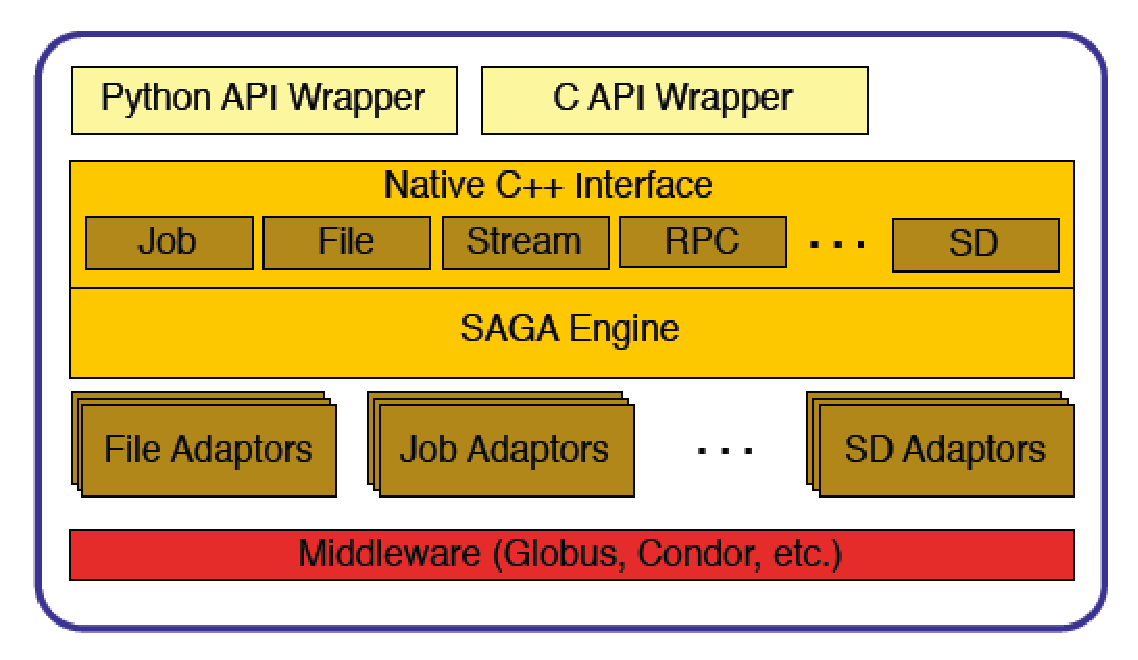
\includegraphics[width=3.55in]{saga_layered_landscape}}     
%     \subfigure{\label{sagalayer2}
%       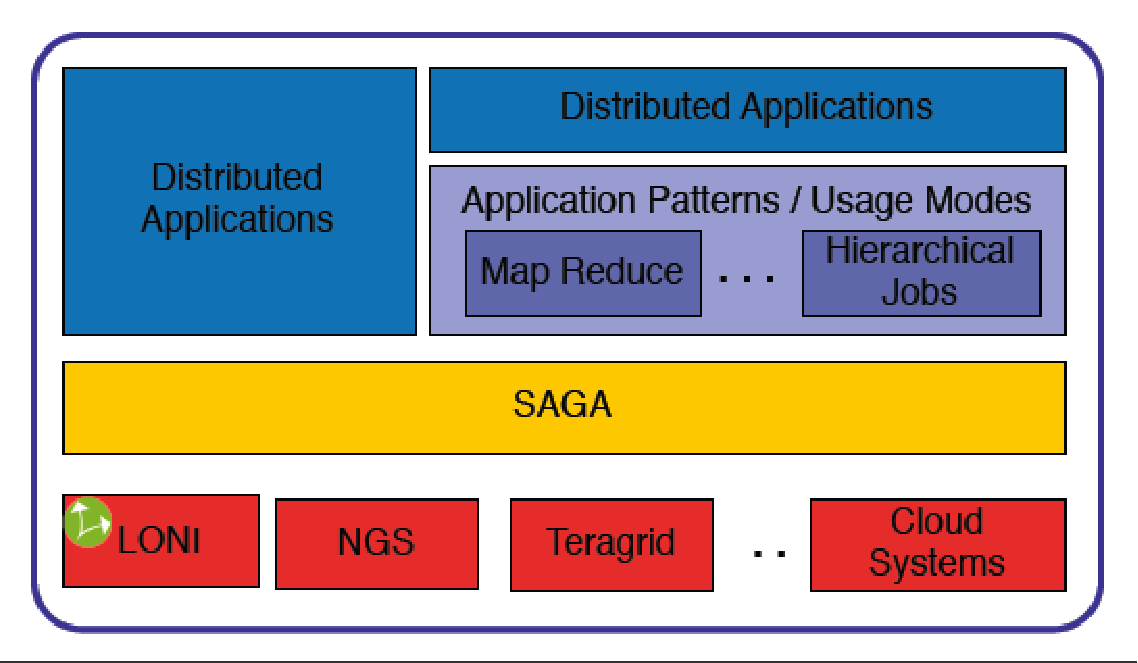
\includegraphics[width=3.55in]{saga_layered_application}}
  \end{center}
  \caption{Layered schematic of the different components of the SAGA
    landscape.  Middleware specific adaptors applications developed
    using SAGA make applications developed using SAGA grid
    portable. Schematic showing the different ways in which SAGA can
    be used to develop distributed applications}
 \label{sagalayer}
\end{figure}


\begin{figure}[!h]
  \begin{center}
%     \subfigure{\label{sagalayer1}
%       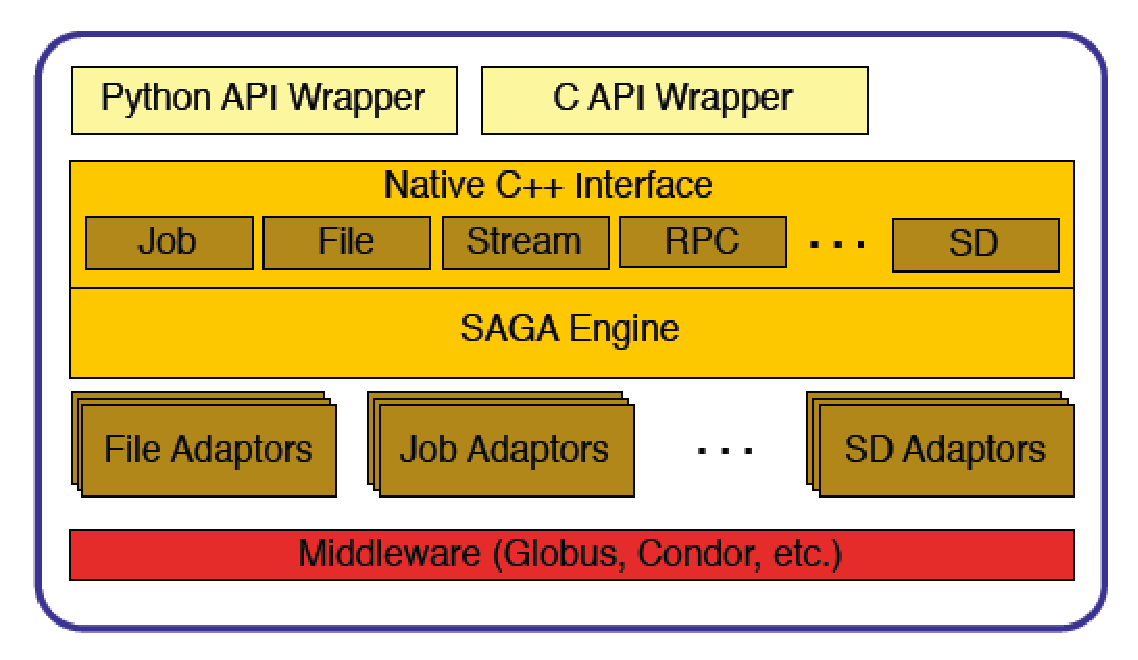
\includegraphics[width=3.55in]{saga_layered_landscape}}     
    \subfigure{\label{sagalayer2}
      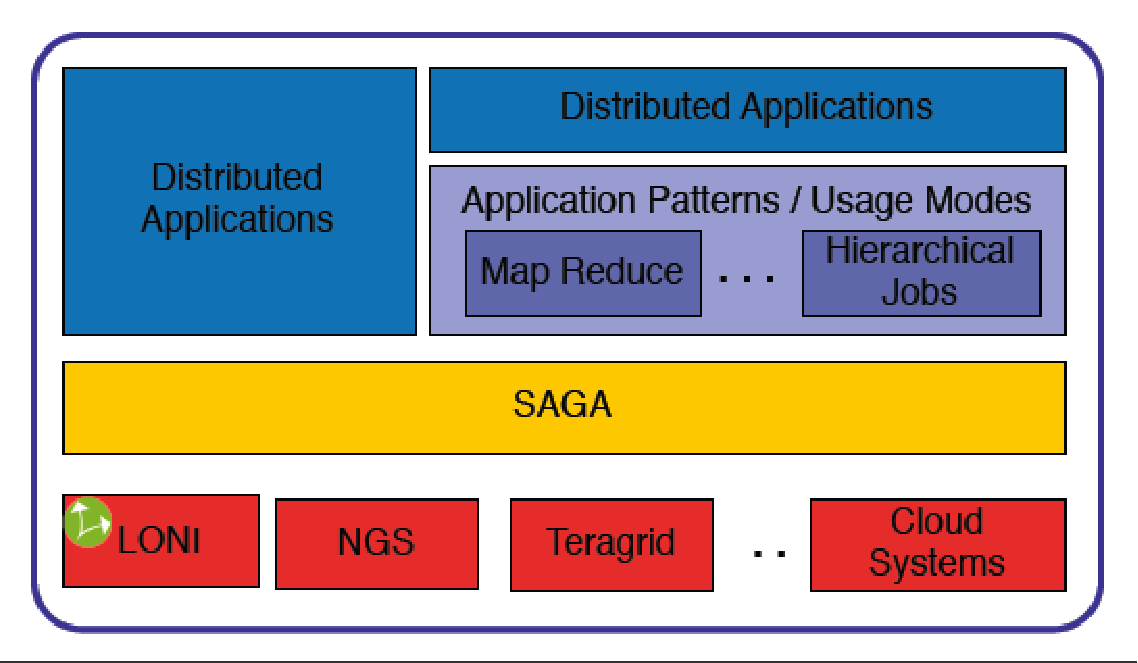
\includegraphics[width=3.55in]{saga_layered_application}}
  \end{center}
  \caption{Layered schematic of the different components of the SAGA
    landscape.  Middleware specific adaptors applications developed
    using SAGA make applications developed using SAGA grid
    portable. Schematic showing the different ways in which SAGA can
    be used to develop distributed applications}
 \label{sagalayer}
\end{figure}


\section{Application With Multiple Loosely-Coupled Homogeneous
  Sub-Tasks}  
\alnote{Are we referring to sub-jobs as sub-tasks or sub-job? Just
to keep this consistent with the other paper. We previously discussed that task
has another meaning within SAGA, which could potentially lead to confusion.}
  
An example for a distributed application consisting of homogeneous sub-tasks
are Replica-Exchange (RE) simulations~\cite{Sugita:1999rm}, \cite{hansmann}. Such applications can be used to understand important
physical phenomena -- ranging from protein folding dynamics to binding
affinity calculations required for computational drug discovery. 
For Replica-Exchange simulations utilizing as many 
distributed resources as possible, is critical for the effective solution of 
the scientific problem.  

Distributed RE simulations must be able to orchestrate different 
resources in a complex and dynamic environment.  Writing
such an applications is a complex task for a myriad number of reasons,
not least of which is that distributed computing environments are
inherently prone to failures. In the following the SAGA-based RE 
framework developed for molecular dynamics simulations
is described.  

\subsection{Application Description}

Replica Exchange simulations are used within Molecular Dynamics (MD) approaches,
to allow a sufficient sampling of configurations. This is
an important requirement for connecting atomistic results to
macroscopic or thermodynamic quantities available from experiments.
However, even with the most powerful computing resources at the
moment, straight-forward MD simulations are unable to reach the
relevant time-scales required to study conformational changes and
searches. This is partly due to the inherent limitations in the MD
algorithm -- a global synchronization is required at the end of each
time step.  This provides an important motivation for research into
finding ways to accelerate sampling and enhance ``effective''
time-scales studied. Generalized ensemble approaches -- of which
Replica-Exchange Molecular Dynamics (REMD)~\cite{Sugita:1999rm} are a
prominent example -- represent an important and promising attempt to
overcome the general limitations of insufficient time-scales, as well
as specific limitations of inadequate conformational sampling arising
from kinetic trappings.  The fact that one single long-running
simulation can be substituted for an ensemble of shorter-running
simulations, make these ideal candidates for distributed environments.

\subsection{Application Architecture}
\alnote{Should I mention CPR/Migol or should I rather keep it on the 
``abstractions'' level?}
Replica-Exchange (RE) simulations can be thought of as consisting of
two distinct components: the  simulation engine/mechanism
used for each replica process, and the coupling-mechanism between the
individual replicas. The RE framework relies NAMD as MD code for 
carrying out the simulation and a SAGA-based framework 
for orchestration of the replica sub-tasks. 

The developed RE framework~\cite{Luckow:2008la} comprises of the \emph{RE-Manager}, the central master 
deployed on the user's desktop, and the  \textit{Replica-Agents}, 
that reside on the High Performance machines where RE simulations
are carried out. The RE-Manager orchestrates all replicas, i.\,e.\ 
it is responsible for the parameterization of replica tasks, 
file staging, job spawning and the conduction of the replica-exchange itself.
The Replica-Agent is launched by a Grid job and is
responsible for spawning and monitoring the replica processes. 

Figure~\ref{fig:remdmanager_v11} summarizes the abstractions used within the RE framework.
For file management the RE-Manager utilizes the SAGA File API. More complex, 
is the management of replica sub-jobs. To achieve an optimal time to solution
an efficient dispatching of the RE sub-jobs is required.  

\begin{figure}[htbp]
    \centering
        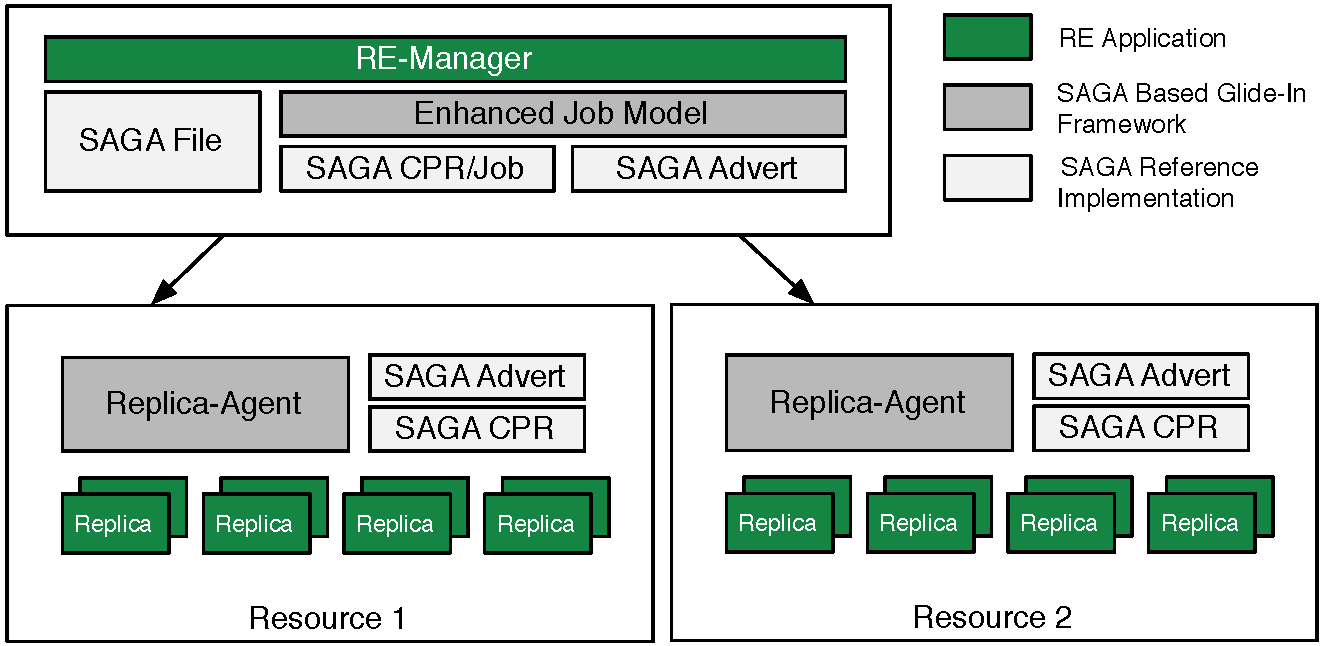
\includegraphics[width=0.45\textwidth]{remdmanager_v11.pdf}
    \caption{Replica Exchange Framework Abstractions:      
          The Replica-Agent is used as placeholder job for
          all replica sub-jobs running on a single cluster. The
          RE-Manager can control both the Replica-Agents and the replica
          jobs using a SAGA-based user-level job API. By using this
          efficient way to allocate resources, queuing times are minimized
          and the time to completion can be dramatically reduced.}
    \label{fig:remdmanager_v11}
\end{figure}  

In particular, queueing delays can represent a major bottleneck: a single crowded 
resource can delay the completion of the simulation arbitrary. A common principle 
to prevent this is the usage of a Glide-In job, which represents a placeholder 
for a set of sub-jobs. For this meta-job a sufficiently large chunk of resources 
is requested. Smaller sub-jobs can then rapidly be executed through the meta-job.

The RE-Manager relies on the SAGA Glide-In framework to efficiently manage both 
Glide-In jobs and sub-jobs. With this capability the SAGA Glide-In framework
provides a novel system-level abstraction for allocating larger chunks of resources 
and for mapping this resources to a set of sub-jobs. The enhanced job model can 
be used as drop-in replacement for a SAGA job objects. No code modification is required
-- the application must solely map the sub-jobs to a larger Glide-In job.

While the implementation of the enhanced job model is entirely based on SAGA 
and in particular the SAGA Advert Service, a central key/value store, a utilization
of other frameworks, such as the orignal Condor Glide-In~\cite{citeulike:291860} or 
Falcon~\cite{1362680}, is possible. Currently, we are actively working on a Condor 
adaptor for SAGA, which will also support native Glide-In functionality for Condor Jobs; 
our enhanced job model 
will then serve as abstraction, while the Condor level Glide-In is used as implementation 
where appropriate. 

\subsection{Deploying on Distributed Resources}

The deployment of the frameworks and application on heterogeneous resources belonging to 
different organizations is a difficult task. In particular, different library 
versions and broken Globus installations led to a high amount of complexity.

\subsection{Deploying in LONI Grid}

To evaluate the performance of the REMD-Manager several
experiments have been conducted on the TeraGrid~\cite{teragrid} and LONI~\cite{loni}. 
The RE-Manager has in particular been tested on QueenBee (QB). 

In particular, the scalability of the Glide-In framework has been extensively tested.
Figure~\ref{fig:perf_remd_glidin} shows that the Glide-In framework is especially 
beneficial if queueing delays occur. The more processes are spawned, the more likely are
such delays. While with the SAGA Glide-In framework the runtime only modestly increase 
with more than 8 replicas, the runtime rapidly rises when using regular Globus job
for spawning NAMD tasks. The unpredictable nature of these queueing times becomes obvious
by the high standard deviation found in the measurements.

\begin{figure}[htbp]
    \centering
        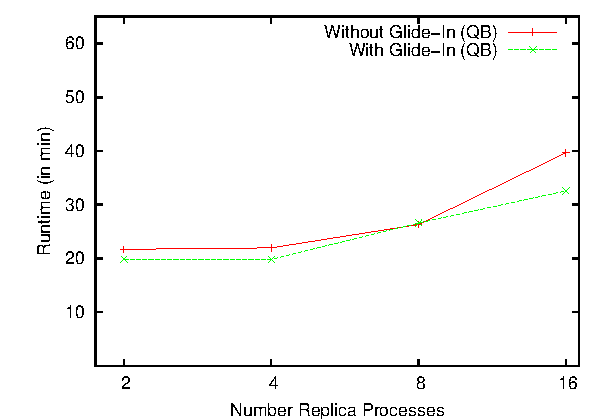
\includegraphics[width=0.5\textwidth]{perf_remd_glidin.pdf}
    \caption{SAGA Glide-In Performance: The usage of the SAGA Glide-In provides a significant reduced time to solution even on a single machine in particular with more than 8 replica jobs.}
    \label{fig:perf_remd_glidin}
\end{figure}


By avoiding long queuing time for big jobs, a distribution of the replica processes to a set 
of less crowded resources provides a lot of benefits.




\section{Applications With Multiple Loosely-Coupled Heterogenous
Sub-Tasks}

\subsection{Application Description}

\subsection{SAGA and Cactus: A Powerful Application Development
  Framework}

\subsection{Deploying on Distributed Resources}

\subsection{Deploying on Ranger}

BQP used for the first time to dynamically determine queue and model
size within a given system to submit sub-task to...


\section{Any Other Applications}

 -- Data parallel applications

\section{Take Home Message}

\begin{itemize}
\item  SAGA provides the ability to create multi-tasks applications that
  can exploit multiple and different infrastructure types.

\item Not only do we need support for different programming models, 
this is also proof of support for agile execution models.

\item We have demonstrated this via the implementation of two
  different applications and running them in two very different
  execution environments.
\end{itemize}







% \Section{Introduction}
%   There exist several applications which require several smaller but
%   heterogenous tasks to be solved in multiple-stages as part of the
%   overall solution.  Often the time-to-solution is the single most
%   important metric.  Distributed resources can thus help, especially
%   when combined with opportunistic scheduling/execution.  However, the
%   desire/need to use distributed computing comes with its own/unique
%   set of challenges.
  
%   We discuss three application types that are in turn composed of
%   multiple, smaller but {\it loosely-coupled} tasks -- Replica
%   Dynamics, Satisfiability problems, and Kalman filtering
%   applications.  Although these applications types are similar in that
%   they are comprised of multiple, smaller tasks, they are different in
%   that the individual sub-tasks are dissimilar for different reasons.
  
%   These application types are often multi-staged, with varying levels
%   of dependency between the stages. There could be, strict ordering
%   between the stages, ie. if all tasks in a stage must complete and be
%   globally synchronised before the next stage can begin. Thus there is
%   coupling between tasks within a given stage, and there is coupling
%   between stages.

%   Other challenges that any many-task system will encounter are: (i)
%   scheduling these sub-tasks is a challenge, (ii) level of speculative
%   computing that can be employed.

%   In parallel replica dynamics, the replicas can run for different
%   time durations between different stages. In replica-exchange
%   dynamics, the number and frequency of exchanges can vary.  Different
%   stages of this application vary; in other words, there is
%   time-domain heterogenity.

%   In Kalman filter based applications, the number and size of 
%   tasks between different stages varies. 

%   In the general class of satisfiability-based applications, as well
%   as the learning-based algorithms, there are elements of both kinds
%   of heterogenity between stages. GridSAT is an interesting example.
         
\newpage
                  
\section*{Acknowledgement}
This work would not have been possible without the efforts and support
of the wider SAGA team. Important funding for SAGA specification and
development has been provided by the UK EPSRC grant number
GR/D0766171/1 (via OMII).  SJ acknowledges the e-Science Institute,
Edinburgh for supporting the research theme, ``Distributed Programming
Abstractions''.  This work has also been made possible thanks to the
internal resources of the Center for Computation \& Technology (CCT)
at Louisiana State University and computer resources provided by LONI.


\bibliographystyle{IEEEtran}
\bibliography{saga,literatur}
\end{document}


